\documentclass[aspectratio=169,11pt,t]{beamer}
% ============================================================
%  ksa-cs-v2: ksa-cs-lecture-template.tex 스타일 + 한글, v2 덱(16:9)용.
%    - 짙은 네이비 헤드라인 (섹션 이름 + 프레임마다 점)
%    - 꽉 찬 파란 제목 막대, 둥근 그림자 블록
%    - 한글: Noto Sans CJK KR (fontspec)
%  사용:
%    \documentclass[aspectratio=169,11pt,t]{beamer}
%    \input{<..>/theme/ksa-cs-v2.tex}
%  ksa-theme.tex 의 매크로(\kb \kq, ksablue/ksared 등)도 같은 이름으로 둔다
%  -> v2 덱 본문을 거의 그대로 옮길 수 있다.
% ============================================================

\usepackage{fontspec}
\usepackage{amsmath,amssymb}
\usepackage{tikz}
\usepackage{listings}
\usepackage{graphicx}
\usepackage{booktabs}
\usepackage{varwidth}
% enumitem 은 넣지 않는다 (beamer 글머리표가 사라진다)

\defaultfontfeatures{Ligatures=TeX}
\setmainfont{Noto Sans CJK KR}
\setsansfont{Noto Sans CJK KR}
\setmonofont{Noto Sans Mono CJK KR}[Scale=0.92]
\usefonttheme{professionalfonts}

% ---------- 기본 틀 ----------
\usetheme{default}
\useinnertheme[shadow=true]{rounded}
\setbeamertemplate{navigation symbols}{}
\setbeamersize{text margin left=1em,text margin right=1em}

% ---------- 색 (템플릿 원본 값) ----------
\definecolor{navydark}{HTML}{191959}
\definecolor{navydim}{HTML}{8888B0}
\definecolor{navytitle}{HTML}{262686}
\definecolor{navyblue}{HTML}{3333B2}
\definecolor{blockbodybg}{HTML}{E9E9F3}
\definecolor{examplegreen}{HTML}{006000}
\definecolor{examplebg}{HTML}{E5EFE5}
\definecolor{alertred}{HTML}{BF0000}
\definecolor{alertbg}{HTML}{F9E5E5}
% ksa-theme.tex 와 같은 이름 (본문 호환)
\colorlet{ksablue}{navytitle}
\colorlet{ksabluedk}{navydark}
\definecolor{ksagold}{HTML}{D6CBB1}
\definecolor{ksagolddk}{HTML}{A9976B}
\colorlet{ksared}{alertred}
\definecolor{ksagray}{HTML}{5B5B5B}

\setbeamercolor{structure}{fg=navyblue}
\setbeamercolor{alerted text}{fg=alertred}
\setbeamercolor{frametitle}{bg=navytitle,fg=white}
\setbeamercolor{title}{fg=white,bg=navytitle}
\setbeamercolor{block title}{bg=navytitle,fg=white}
\setbeamercolor{block body}{bg=blockbodybg,fg=black}
\setbeamercolor{block title example}{bg=examplegreen,fg=white}
\setbeamercolor{block body example}{bg=examplebg,fg=black}
\setbeamercolor{block title alerted}{bg=alertred,fg=white}
\setbeamercolor{block body alerted}{bg=alertbg,fg=black}
\setbeamercolor{item}{fg=navyblue}
\setbeamertemplate{itemize item}[circle]
\setbeamertemplate{itemize subitem}[triangle]

% ---------- 헤드라인: miniframes (섹션 이름 + 점) ----------
\useoutertheme[subsection=false]{miniframes}
\setbeamerfont{section in head/foot}{size=\tiny}
\setbeamercolor{section in head/foot}{bg=navydark,fg=white}
\setbeamercolor{mini frame}{fg=white}
\setbeamertemplate{mini frames}[circle]

% ---------- 제목 막대: 폭 꽉 채움, 두 줄까지 ----------
\setbeamerfont{frametitle}{size=\normalsize,series=\bfseries}
\setbeamertemplate{frametitle}{%
  \nointerlineskip
  \begin{beamercolorbox}[wd=\paperwidth,ht=2.7ex,dp=1.1ex,leftskip=.3cm,rightskip=.3cm]{frametitle}%
    \usebeamerfont{frametitle}\insertframetitle
  \end{beamercolorbox}}

% ---------- 쪽 번호: 오른쪽 아래 ----------
\setbeamertemplate{footline}{%
  \hfill
  {\color{navydim}\scriptsize\insertframenumber\,/\,\inserttotalframenumber}%
  \hspace{3mm}\vspace{2mm}%
}

% ---------- 표지: 템플릿처럼 헤드라인은 그대로, 가운데 둥근 그림자 상자에 제목 한 줄 ----------
% 덱에서:  {\setbeamertemplate{footline}{}\begin{frame}[c,noframenumbering]\titlepage\end{frame}}
\setbeamercolor{title}{fg=white,bg=navyblue}
\makeatletter
\setbeamertemplate{title page}{%
  \vfill
  \centering
  \begin{minipage}{0.84\paperwidth}
  \begin{beamercolorbox}[wd=\linewidth,sep=7pt,center,rounded=true,shadow=true]{title}
    {\usebeamerfont{title}\inserttitle\par}%
    \ifx\insertsubtitle\@empty\else\vskip0.4em{\usebeamerfont{subtitle}\insertsubtitle\par}\fi
  \end{beamercolorbox}
  \end{minipage}\par\vskip1.6em
  {\usebeamerfont{author}\color{navytitle}\insertauthor\par}\vskip0.3em
  {\usebeamerfont{institute}\color{ksagray}\insertinstitute\par}
  \vfill
}
\makeatother
\setbeamerfont{title}{series=\bfseries,size=\Large}
\setbeamerfont{subtitle}{size=\normalsize}
\setbeamerfont{author}{size=\normalsize}
\setbeamerfont{institute}{size=\small}

% ksa-theme 호환: 덱이 \renewcommand{\ksacredit}{..} 를 해도 되게 (꼬리말에는 안 쓴다)
\newcommand{\ksacredit}{}

% ---------- 강조 ----------
\newcommand{\hl}[1]{\textcolor{alertred}{#1}}
\newcommand{\hlb}[1]{\textcolor{navyblue}{#1}}
\newcommand{\kb}[1]{\textbf{\color{ksablue}#1}}
\newcommand{\kq}[1]{\textbf{\color{ksared}#1}}

% ---------- 파이썬 코드 (템플릿과 같은 색) ----------
\definecolor{codekw}{HTML}{0033B3}
\definecolor{codebuiltin}{HTML}{BF0000}
\definecolor{codestr}{HTML}{067D17}
\definecolor{codecomment}{HTML}{8C8C8C}
\definecolor{codenum}{HTML}{1750EB}
\lstdefinestyle{py}{
  language=Python, basicstyle=\ttfamily\scriptsize,
  keywordstyle=\color{codekw}\bfseries, stringstyle=\color{codestr},
  commentstyle=\color{codecomment}\itshape, numberstyle=\color{codenum},
  emph={print,len,range,sum,input,int,str,float,list,dict,append,remove,sorted,abs,min,max},
  emphstyle=\color{codebuiltin}, showstringspaces=false, keepspaces=true,
  columns=fixed, basewidth=0.52em, aboveskip=1mm, belowskip=1mm, xleftmargin=2mm,
  breaklines=true
}
\lstset{style=py}

% 원본 덱 (ksa-theme): slides/v2/ml1/week02/pr_auc/ -- 그림은 거기 figs/ 를 그대로 쓴다
\setbeamerfont{author}{size=\normalsize}
\setbeamerfont{institute}{size=\small}
\graphicspath{{../../../v2/ml1/week02/pr_auc/figs/}{../../../assets/}}
\makeatletter
\newcommand{\markpage}[1]{\protected@write\@auxout{}{\string\newlabel{#1}{{\the\c@framenumber}{}}}\hypertarget{#1}{}}
\newcommand{\pref}[1]{\hyperlink{#1}{\textcolor{ksagolddk}{(p.\ref{#1})}}}
\makeatother

\renewcommand{\ksacredit}{Machine Learning and Deep Learning \,\textperiodcentered\, ROC-AUC와 PR-AUC}
\title{ROC-AUC와 PR-AUC}
\subtitle{기준선 하나가 아니라, 기준선 전체로 평가하기}
\author{Machine Learning and Deep Learning}
\institute{한국과학영재학교 (KSA)}
\date{}
\begin{document}
{\setbeamertemplate{footline}{}\begin{frame}[c,noframenumbering]\titlepage\end{frame}}

\section{질문}
% --- 오늘의 질문
\begin{frame}{오늘의 질문}
\vfill
\centering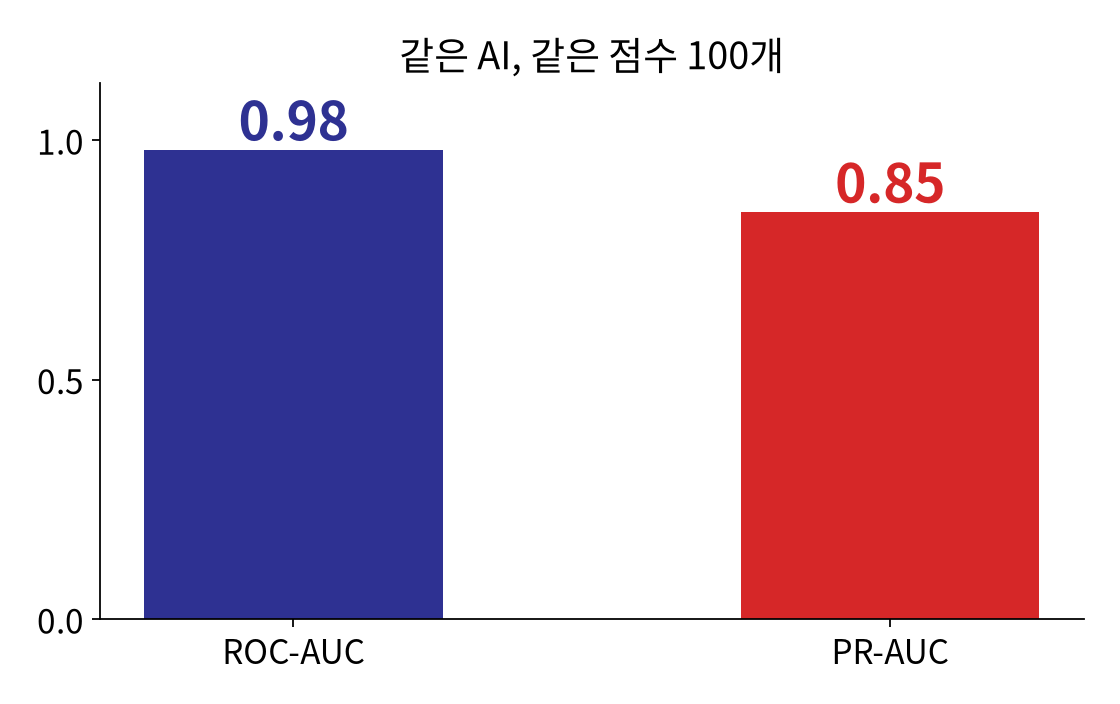
\includegraphics[width=0.5\linewidth]{pa_hook.png}\par\vskip0.3em
{\large 지난 시간의 독감 AI (100명 중 독감 10명).\\ \kq{같은 AI 인데 왜 0.98 과 0.85 로 다를까?}}
\vfill
\note{지난 시간의 독감 AI입니다. 학교 100명 중 독감 10명이고, AI는 학생마다 독감일 확률 점수를 냅니다. 이 AI를 평가하는 대표적인 점수가 두 개 있는데, 하나는 0.98, 다른 하나는 0.85가 나옵니다. 같은 AI, 같은 점수 100개인데 왜 이렇게 다를까요? 어느 쪽을 믿어야 할까요? 오늘은 이 두 점수가 각각 무엇을 재는지 알아봅니다.}
\end{frame}

\section{ROC}
% --- 기준선 하나 = 점 하나
\begin{frame}{기준선 하나로는 부족하다}
\vfill
\centering
{\Large 기준 0.5 \quad $\to$ \quad 정밀도 67\% · 재현율 80\%}\\[0.8em]
{\Large 기준 0.7 \quad $\to$ \quad 정밀도 86\% · 재현율 60\%}\\[1.2em]
{\large 기준을 바꿀 때마다 성적이 달라진다 \quad $\to$ \kb{모든 기준을 한꺼번에} 평가하고 싶다}\\[0.6em]
{\small 기준을 1 에서 0 까지 내리며 찍은 점들을 이으면 곡선, 그 아래 넓이가 \textbf{AUC} (area under the curve)}
\vfill
\note{지난 시간에 본 것처럼 기준선을 0.5에 두면 정밀도 67, 재현율 80이고, 0.7로 올리면 86과 60이 됩니다. 기준을 어디에 두느냐에 따라 성적이 달라지니, 기준 하나로 AI를 평가하면 공정하지 않습니다. 기준은 나중에 문제에 맞춰 정하면 되니까, AI 자체의 실력은 모든 기준을 한꺼번에 보고 평가하고 싶습니다. 방법은 기준을 1에서 0까지 내리며 성적을 점으로 찍고, 점들을 이은 곡선 아래의 넓이를 재는 것입니다. 이 넓이를 AUC, area under the curve라고 부릅니다. 어떤 성적을 찍느냐에 따라 ROC와 PR, 두 가지가 있습니다.}
\end{frame}

% --- ROC 곡선
\begin{frame}{ROC 곡선: 헛짚음 비율 vs 재현율}
\markpage{roc}
\vfill
\begin{columns}[c]
\begin{column}{0.46\textwidth}\centering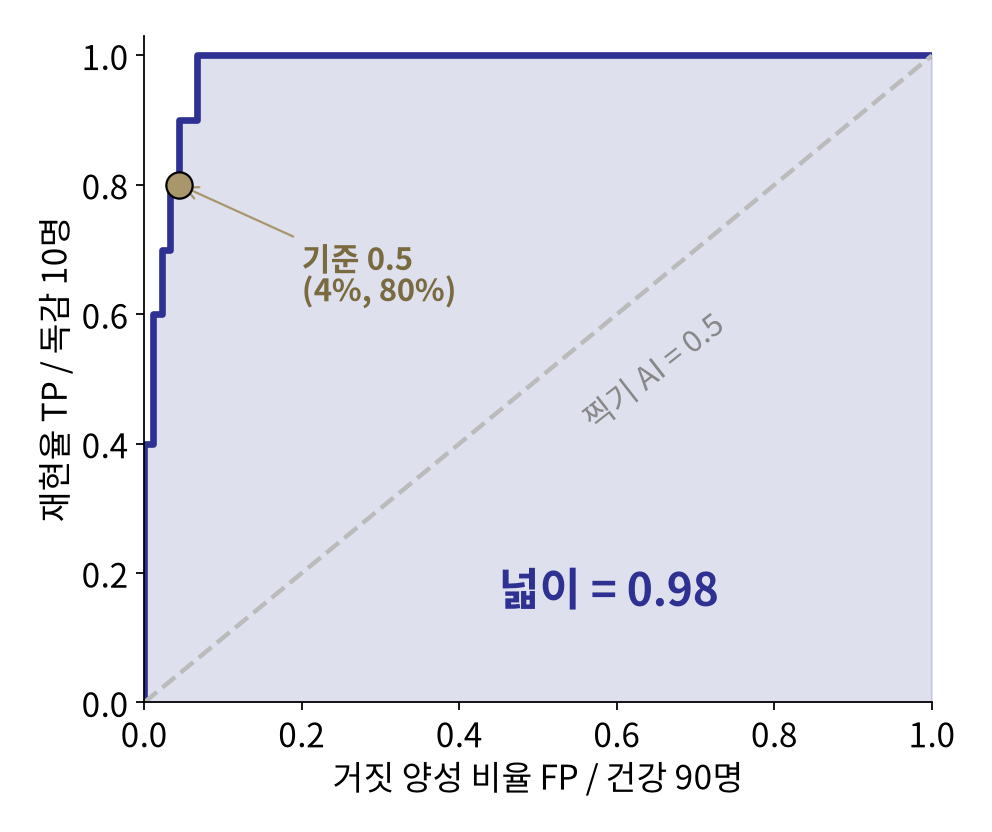
\includegraphics[width=\linewidth]{pa_roc.png}\end{column}
\begin{column}{0.5\textwidth}
{\large 가로 \quad $\text{FPR} = \dfrac{FP}{FP + TN}$}\\[0.2em]
{\small 건강한 90명 중 ``독감''이라고 헛짚은 비율}\\[0.8em]
{\large 세로 \quad $\text{TPR} = \dfrac{TP}{TP + FN}$}\\[0.2em]
{\small 독감 10명 중 찾아낸 비율 = 재현율}\\[0.8em]
{\large 기준 0.5: \; $\left(\tfrac{4}{90},\ \tfrac{8}{10}\right) = (4\%,\ 80\%)$}
\end{column}
\end{columns}
\vfill
\note{첫 번째는 ROC 곡선입니다. 가로축은 거짓 양성 비율, FPR입니다. 건강한 90명 중 독감이라고 헛짚은 비율입니다. 세로축은 재현율, 독감 10명 중 찾아낸 비율이고 ROC에서는 TPR이라고도 부릅니다. 기준 0.5에서는 헛짚은 학생이 4명이니 90명 중 4명, 4퍼센트이고, 재현율은 80퍼센트라 노란 점입니다. 기준을 1에서 0으로 내리면 왼쪽 아래 (0, 0)에서 출발해 오른쪽 위 (1, 1)로 가는 계단이 생깁니다. 독감 학생을 찾으면 위로, 헛짚으면 오른쪽으로 한 칸씩 갑니다.}
\end{frame}

% --- ROC-AUC
\begin{frame}{ROC-AUC = 짝 비교에서 이긴 비율}
\vfill
\centering
{\LARGE\[ \text{ROC-AUC} = \frac{\text{독감 점수} > \text{건강 점수 인 짝}}{\text{독감 10} \times \text{건강 90}} = \frac{883}{900} = 0.98 \]}\vskip0.6em
{\large 독감 학생 하나, 건강 학생 하나를 뽑으면 \kb{독감 학생의 점수가 더 높을 확률}}\\[0.8em]
{\small 찍기 AI (점수가 무작위) $\to$ 반반 $\to$ 0.5 \qquad 완벽한 AI $\to$ 1}
\vfill
\note{ROC 곡선 아래 넓이를 ROC-AUC라고 합니다. 넓이를 직접 적분해도 되지만, 더 쉬운 해석이 있습니다. 독감 학생 10명과 건강 학생 90명으로 짝을 만들면 900쌍입니다. 그중 독감 학생의 점수가 더 높은 짝을 세면 883쌍, 883 나누기 900이 0.98입니다. 이 값이 정확히 ROC 곡선 아래 넓이와 같습니다. 즉 ROC-AUC는 독감 학생과 건강 학생을 하나씩 뽑았을 때 AI가 독감 학생에게 더 높은 점수를 줄 확률입니다. 점수를 아무렇게나 주는 찍기 AI는 반반이니 0.5, 완벽한 AI는 1입니다.}
\end{frame}

\section{PR}
% --- ROC 가 너그러운 이유
\begin{frame}{같은 헛짚음 4명, 무엇으로 나누나}
\markpage{divide}
\vfill
\centering
{\LARGE\[ \underbrace{\frac{4}{90} = 4\%}_{\text{ROC: 건강 90명으로}} \qquad\qquad \underbrace{\frac{4}{12} = 33\% \;\text{틀림}}_{\text{PR: AI 가 고른 12명으로}} \]}\vskip0.8em
{\large ROC 는 건강한 학생이 많을수록 헛짚음이 \kq{작아 보인다}}\\[0.4em]
{\large 하지만 ``독감''이라는 AI 말은 3번 중 1번 틀렸다 \quad (정밀도 67\%)}
\vfill
\note{기준 0.5에서 헛짚은 학생은 4명입니다. ROC는 이 4명을 건강한 학생 90명으로 나눠서 4퍼센트라고 합니다. 아주 작아 보입니다. 그런데 AI가 독감이라고 한 학생은 12명이고, 그중 4명이 틀렸습니다. AI가 독감이라고 말하면 3번 중 1번은 틀린다는 뜻이고, 정밀도로 말하면 67퍼센트입니다. 같은 4명인데 무엇으로 나누느냐에 따라 4퍼센트와 33퍼센트로 달라집니다. 건강한 학생이 많은 쏠린 데이터일수록 ROC는 헛짚음을 작게 보이게 합니다.}
\end{frame}

% --- PR 곡선
\begin{frame}{PR 곡선: 재현율 vs 정밀도}
\markpage{pr}
\vfill
\begin{columns}[c]
\begin{column}{0.46\textwidth}\centering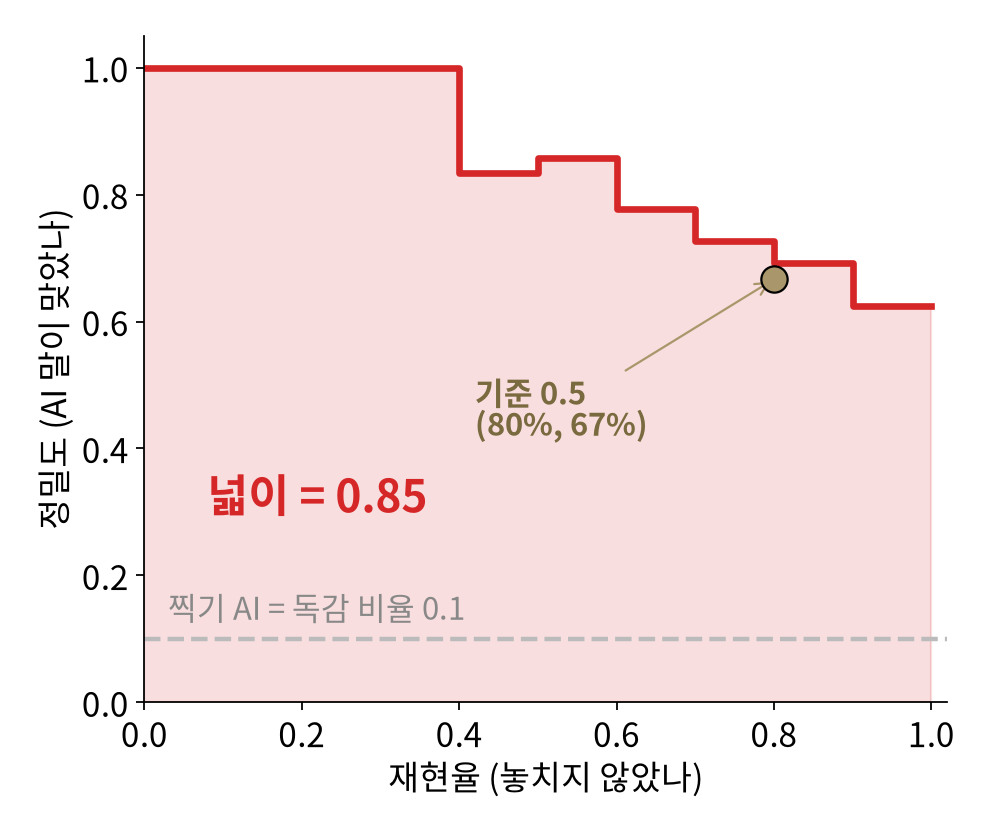
\includegraphics[width=\linewidth]{pa_pr.png}\end{column}
\begin{column}{0.5\textwidth}
{\large 가로 \quad 재현율 $\dfrac{TP}{TP + FN}$}\\[0.2em]
{\small 놓치지 않았나?}\\[0.8em]
{\large 세로 \quad 정밀도 $\dfrac{TP}{TP + FP}$}\\[0.2em]
{\small AI 말이 맞았나?}\\[0.8em]
{\large 기준 0.5: \; $(80\%,\ 67\%)$}
\end{column}
\end{columns}
\vfill
\note{두 번째는 PR 곡선입니다. 가로축은 재현율, 세로축은 정밀도입니다. 지난 시간의 두 지표를 그대로 축으로 쓴 겁니다. 기준 0.5는 재현율 80, 정밀도 67인 노란 점입니다. 기준을 내리면 재현율은 오른쪽으로 늘고, 헛짚음이 섞이면서 정밀도는 내려갑니다. ROC 곡선과 달리 헛짚음을 AI가 고른 학생 수로 나누기 때문에, 건강한 학생이 아무리 많아도 헛짚음이 작아 보이지 않습니다.}
\end{frame}

% --- 줄 세워 세기
\begin{frame}{PR-AUC 를 직접 세기: 점수 순으로 줄 세우기}
\markpage{rank}
\vfill
\centering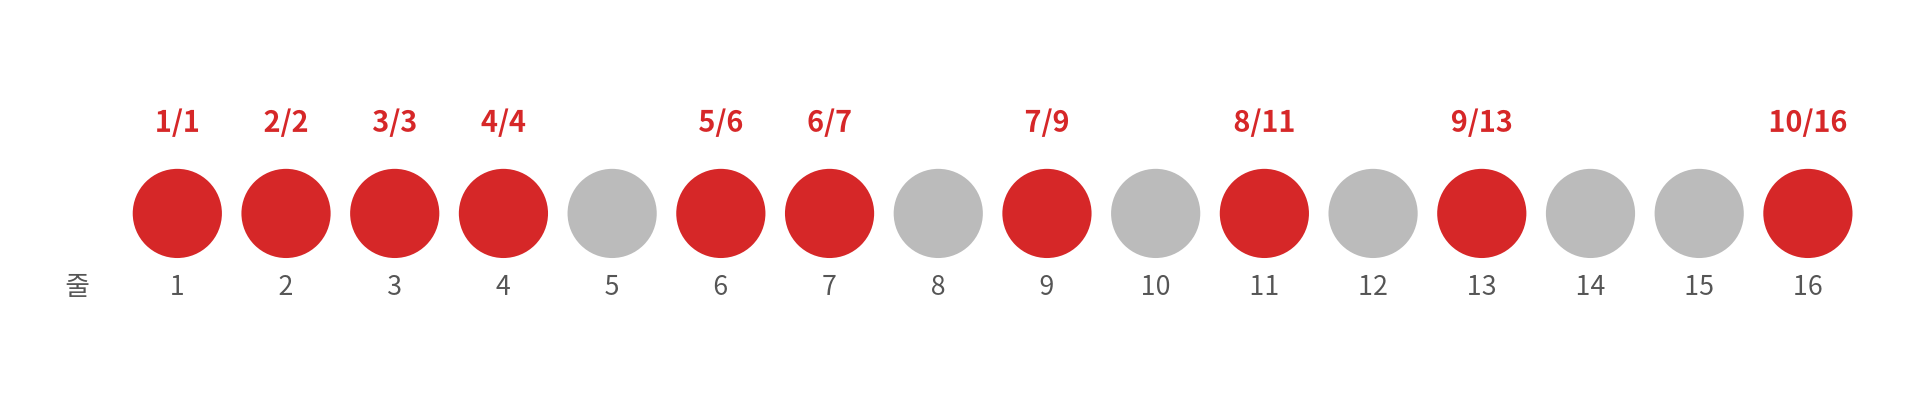
\includegraphics[width=0.94\linewidth]{pa_rank.png}\par\vskip0.3em
{\large 독감 학생(빨강)을 찾을 때마다 그때까지의 정밀도를 적는다}\\[0.5em]
{\large $\dfrac{1}{1}, \dfrac{2}{2}, \dfrac{3}{3}, \dfrac{4}{4}, \dfrac{5}{6}, \dfrac{6}{7}, \dfrac{7}{9}, \dfrac{8}{11}, \dfrac{9}{13}, \dfrac{10}{16}$}
\vfill
\note{PR 곡선 아래 넓이를 직접 세어 봅니다. 학생 100명을 점수가 높은 순서로 줄 세웠습니다. 위 16명만 보이는데, 빨강이 독감, 회색이 건강입니다. 줄의 앞에서부터 한 명씩 독감이라고 판정해 나간다고 생각하세요. 독감 학생을 찾을 때마다 그때까지의 정밀도를 적습니다. 1, 2, 3, 4번째는 모두 독감이라 1/1부터 4/4까지 모두 100퍼센트입니다. 5번째에 처음 헛짚고, 6번째에 다섯 번째 독감을 찾으니 5/6입니다. 이렇게 마지막 열 번째 독감 학생은 16번째에 나와서 10/16입니다.}
\end{frame}

% --- AP
\begin{frame}{PR-AUC = 그 정밀도들의 평균}
\vfill
\centering
{\Large\[ \text{PR-AUC} = \frac{1}{10}\left(1 + 1 + 1 + 1 + \frac{5}{6} + \frac{6}{7} + \frac{7}{9} + \frac{8}{11} + \frac{9}{13} + \frac{10}{16}\right) = 0.85 \]}\vskip0.6em
{\large 독감 학생을 찾을 때마다의 정밀도를 평균 = \kb{Average Precision (AP)}}\\[0.6em]
{\small 재현율이 0.1 씩 오를 때마다 그때의 정밀도를 높이로 하는 막대 10개의 넓이 = PR 곡선 아래 넓이 \pref{pr}}
\vfill
\note{적어 둔 정밀도 10개를 평균 내면 0.85입니다. 이것이 PR-AUC이고, 정확한 이름은 평균 정밀도, Average Precision, 줄여서 AP입니다. 왜 이게 곡선 아래 넓이일까요? 독감 학생을 하나 찾을 때마다 재현율이 10분의 1씩 오릅니다. 그러면 PR 곡선 아래는 폭 0.1, 높이가 그때의 정밀도인 막대 10개로 나뉘고, 넓이를 더하면 정밀도 10개의 평균과 같습니다. 앞쪽에서 헛짚을수록, 즉 건강한 학생에게 높은 점수를 줄수록 평균이 떨어집니다.}
\end{frame}

\section{비교}
% --- 찍기 AI
\begin{frame}{찍기 AI 의 점수도 다르다}
\vfill
\centering
{\Large\begin{tabular}{lcc}
 & ROC-AUC & PR-AUC\\\hline\\[-0.8em]
찍기 AI (무작위 점수) & 0.5 & \kq{0.1 (독감 비율)}\\[0.3em]
우리 AI & 0.98 & 0.85\\[0.3em]
완벽한 AI & 1 & 1
\end{tabular}}\vskip1.0em
{\large 바닥이 다르다: \quad ROC-AUC 는 0.5 부터, \quad PR-AUC 는 0.1 부터}
\vfill
\note{두 점수는 바닥도 다릅니다. 점수를 아무렇게나 주는 찍기 AI는 ROC-AUC가 0.5입니다. 반면 PR-AUC는 독감 비율인 0.1 근처입니다. 무작위로 골라도 정밀도는 대략 독감 비율만큼 나오니까요. 그래서 0.98과 0.85를 그대로 비교하면 안 됩니다. ROC-AUC는 0.5에서 시작하는 점수이고, PR-AUC는 0.1에서 시작하는 점수입니다. 독감이 1퍼센트뿐인 데이터라면 PR-AUC의 바닥은 0.01이 됩니다.}
\end{frame}

% --- 건강 10배
\begin{frame}{건강한 학생이 10배가 되면}
\markpage{x10}
\vfill
\centering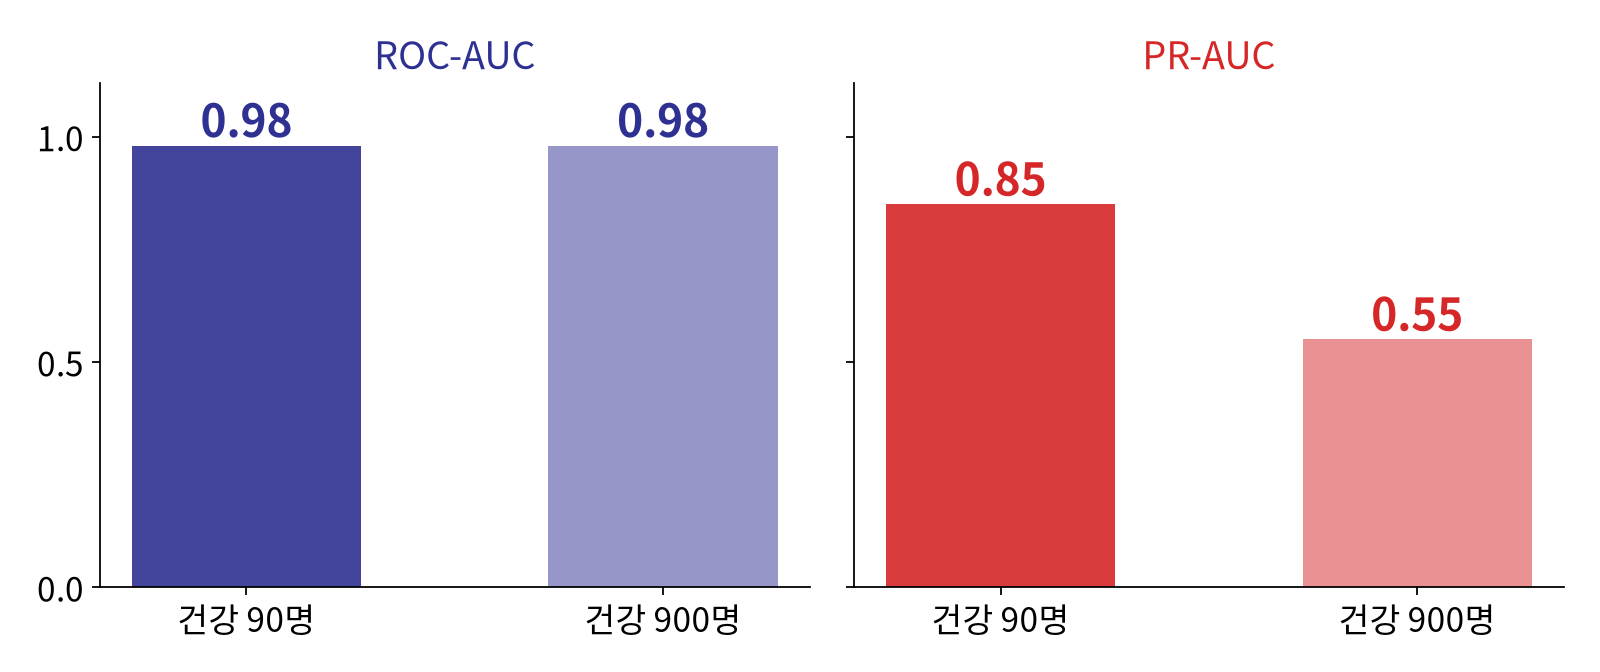
\includegraphics[width=0.66\linewidth]{pa_x10.png}\par\vskip0.3em
{\large 같은 점수의 건강 학생을 10배로 \quad ROC-AUC \kb{0.98 그대로} \quad PR-AUC \kq{0.85 $\to$ 0.55}}\\[0.3em]
{\small 헛짚는 학생 수도 10배 $\to$ AI 의 ``독감'' 판정은 훨씬 자주 틀린다. ROC 는 비율이라 못 느낀다}
\vfill
\note{더 쏠린 데이터를 만들어 봅니다. 독감 학생은 그대로 10명, 건강한 학생은 같은 점수를 가진 학생을 10배로 늘려 900명으로 만들었습니다. AI의 실력은 똑같습니다. ROC-AUC는 0.98 그대로입니다. 짝 비교에서 이기는 비율이 바뀌지 않으니까요. 하지만 PR-AUC는 0.55로 떨어집니다. 건강한 학생이 10배면 헛짚는 학생도 10배라서, AI가 독감이라고 할 때 틀리는 경우가 훨씬 많아지기 때문입니다. 실제로 병원에서 이 AI를 쓰는 사람이 느끼는 것은 PR-AUC 쪽입니다.}
\end{frame}

% --- 언제 무엇을
\begin{frame}{언제 무엇을 볼까}
\vfill
\centering
\renewcommand{\arraystretch}{1.5}
{\large\begin{tabular}{lll}
\kb{ROC-AUC} & 두 쪽이 비슷하게 많을 때 & 쏠림에 둔하다 (너그러움)\\
\kq{PR-AUC} & 찾을 것이 드물 때 (사기 · 희귀병) & 쏠림을 반영 (엄격함)
\end{tabular}}\vskip1.0em
{\large 쏠린 데이터라면 \textbf{둘 다} 적고, PR-AUC 는 \textbf{바닥(양성 비율)과 함께} 적는다}
\vfill
\note{정리하면, ROC-AUC는 양성과 음성을 얼마나 잘 줄 세우는지를 보는 점수라서 데이터가 쏠려도 크게 변하지 않습니다. 그 대신 쏠린 데이터에서는 너무 좋아 보일 수 있습니다. PR-AUC는 AI가 양성이라고 한 말이 얼마나 맞는지를 보기 때문에 쏠림을 그대로 반영합니다. 사기 거래, 희귀병, 스팸처럼 찾을 것이 드문 문제에서는 PR-AUC를 꼭 같이 봅니다. 논문이나 보고서에서는 둘 다 적고, PR-AUC는 바닥인 양성 비율을 함께 적어야 읽는 사람이 판단할 수 있습니다.}
\end{frame}

\section{연습}
% --- 문제풀이
\begin{frame}{문제풀이}
\vfill
\begin{enumerate}
\item 양성 2명(점수 0.9, 0.4), 음성 3명(0.8, 0.3, 0.2). \; (a) 짝 6개 중 양성이 이긴 짝은? ROC-AUC 는? \; (b) 줄 세워 AP 를 구하면?\vskip0.8em
\item 양성 비율이 5\% 인 데이터에서 어떤 모델의 PR-AUC 가 0.30 이다. 좋은 모델인가?\vskip0.8em
\item 음성 데이터만 100배로 늘렸다 (모델은 그대로). ROC-AUC 와 PR-AUC 는 각각 어떻게 되나?
\end{enumerate}
\vfill
\note{1번 답. 0.9는 음성 셋을 모두 이기고, 0.4는 0.3과 0.2를 이겨서 6쌍 중 5쌍, ROC-AUC는 6분의 5, 약 0.83입니다. 줄 세우면 0.9 양성, 0.8 음성, 0.4 양성 순서라서, 첫 양성에서 정밀도 1/1, 두 번째 양성에서 2/3, 평균 AP는 약 0.83입니다. 2번 답. 바닥이 0.05니까 0.30은 찍기보다 6배 높은 정밀도 수준입니다. 문제에 따라 쓸모 있을 수 있고, 0.3이라는 숫자만 보고 나쁘다고 하면 안 됩니다. 3번 답. ROC-AUC는 그대로, PR-AUC는 떨어집니다.}
\end{frame}

% --- 실습
\begin{frame}{실습}
\vfill
\centering\begin{tabular}{rl}
\large 1 & 슬라이드의 점수 100개로 ROC-AUC (짝 세기) · AP (줄 세우기) 구현 $\to$ 0.98 · 0.85\\[0.5em]
\large 2 & 건강 학생을 10배 · 100배로 늘리며 두 점수 비교\\[0.5em]
\large 3 & 실제 데이터: 오존 경보 (양성 6\%), 두 모델을 ROC-AUC 와 PR-AUC 로 비교
\end{tabular}\vskip1em
Ozone Level Detection (UCI; OpenML) \\[0.4em]\href{https://colab.research.google.com/github/SuminHan/book-ml/blob/main/slides/v2/ml1/week02/pr_auc/lab/pr_auc.ipynb}{\textcolor{ksagolddk}{▶ Colab에서 실습 노트북 열기}}
\vfill
\note{실습은 세 부분입니다. 첫째, 슬라이드의 점수 100개로 ROC-AUC를 짝 세기로, AP를 줄 세우기로 직접 구현해서 0.98과 0.85를 재현하고 scikit-learn과 비교합니다. 둘째, 건강한 학생을 10배, 100배로 늘리며 두 점수가 어떻게 변하는지 봅니다. 셋째, 휴스턴의 날씨 측정값으로 오존 경보일을 예측하는 실제 데이터에서, 양성이 6퍼센트뿐일 때 두 모델을 ROC-AUC와 PR-AUC로 비교합니다.}
\end{frame}

\section{정리}
% --- 정리
\begin{frame}{정리}
\vfill
\centering\large\begin{tabular}{l}
기준을 1 $\to$ 0 으로 내리며 찍은 곡선의 넓이 = \textbf{AUC}\\[0.5em]
\kb{ROC-AUC} \quad 독감 학생이 건강 학생보다 점수가 높을 확률 (찍기 = 0.5)\\[0.5em]
\kq{PR-AUC (AP)} \quad 독감 학생을 찾을 때마다의 정밀도 평균 (찍기 = 양성 비율)\\[0.5em]
쏠린 데이터: ROC 는 너그럽고 PR 은 엄격하다 $\to$ 둘 다 본다
\end{tabular}
\vfill
\note{정리합니다. 기준을 1에서 0까지 내리며 찍은 점들을 이은 곡선 아래 넓이가 AUC입니다. ROC-AUC는 독감 학생과 건강 학생을 하나씩 뽑았을 때 독감 학생 점수가 더 높을 확률이고, 찍기 AI는 0.5입니다. PR-AUC, 즉 AP는 점수 순으로 줄 세워 독감 학생을 찾을 때마다의 정밀도를 평균 낸 것이고, 찍기 AI는 양성 비율입니다. 쏠린 데이터에서 ROC는 너그럽고 PR은 엄격하니, 둘 다 보는 습관을 들입시다.}
\end{frame}
\end{document}
